% vim: set spell:
% vim: set spell spelllang=en:
\documentclass[a4paper,10pt]{article}
%\usepackage[mathjax]{lwarp}
%\usepackage{lwarp}
\usepackage[utf8]{inputenc}
\usepackage{tikz}
\usepackage[T1]{fontenc}
\usepackage{amsfonts}
\usepackage{amsmath}
\usepackage{pifont}
\usepackage{tikz}
\usetikzlibrary{calc}
\usepackage{hyperref}
\usepackage{stmaryrd}
\usepackage[left=2cm,right=2cm]{geometry}
\usepackage{listings}

\title{Tutorials : Concepts of Logic and Programming}
\author{Nicolas González}
\date{October 7th 2020}

\def\centralruler{\begin{center}\rule{5cm}{.1pt}\end{center}}

\newcommand{\R}{\mathbb{R}}
\newcommand{\Com}{\mathbb{C}}
\newcommand{\K}{\mathbb{K}}
\newcommand{\Z}{\mathbb{Z}}
\newcommand{\N}{\mathbb{N}}
\newcommand{\Lin}{\mathcal{L}}
\newcommand{\Mnn}{\mathcal{M}_n(\R)}
\newcommand{\ProScal}[2]{\langle #1,#2 \rangle}
\newcommand{\Norm}[1]{\left|\left| #1 \right|\right|}
\newcommand{\grad}{\overrightarrow{\nabla}}
\newcommand{\Proba}{\mathbb{P}}
\newcommand{\vv}[1]{\overrightarrow{\textbf{#1}}}

\DeclareMathOperator{\Vect}{Vect}
\DeclareMathOperator{\Imag}{\Im m}
\DeclareMathOperator{\Mat}{Mat}
\DeclareMathOperator{\rk}{rk}
\DeclareMathOperator{\asinh}{asinh}


\renewcommand{\theequation}{\thesubsection--\arabic{equation}}


\newcommand{\Tstrut}{\rule{0pt}{2.6ex}}
\newcommand{\Bstrut}{\rule[-0.9ex]{0pt}{0pt}}
\newcommand{\TBstrut}{\Tstrut\Bstrut}
%\usepackage[toc]{glossaries}
%\makeglossaries
%\loadglsentries{glossary}

\begin{document}

\maketitle

This document is meant as a repository of my works for the tutorials of ``Concepts from Logic to Programming'', specifically the fifth tutorial. The content is essentially my work for these tutorials, and is fallible, and contains errors. If you find any, or you have questions or you're missing files, send me an email at \textit{Nicolas.Gonzalez@insa-rennes.fr}, and I will get back to you.

%\tableofcontents

\newpage

\section{Exercice}

\underline{\textbf{Problème :}}
On souhait créer un circuit permettant de calculer les termes de la suite de Fibonacci. La formule de réucurrence de cette suite est la suivante :
\begin{align*}
	\mathbb{F}_0&=0\\
	\mathbb{F}_1&=1\\
	\forall n\in\N,\ n>1,\quad\mathbb{F}_n&=\mathbb{F}_{n-1}+\mathbb{F}_{n-2}
\end{align*}

Afin de calculer ces différents termes, on se base sur l'algorithme suivant :
\begin{lstlisting}
Faire
	Tant que NOT init faire
		N0 = 0 ;
		N1 = 1 ;
		N = n ;
		Q = 0 ;
		Res = 0 ;
	Fait
	Tant que N > Q faire
		N1 = N0 + N1, N0 = N1 ;
		Q = Q+1 ;
	Fait
	Tant que init faire
		Res = 1 ;
		Afficher(N0) ;
	Fait
		Res = 0 ;
Fait
\end{lstlisting}

(NDLR: J'ai dû modifier le pseudocode légèrement pour accomoder l'impossibilité de formatter des expressions mathématiques dans les listings de code \LaTeX.)

\textbf{Attention!} la partie de code en gras (boucle tant que $N>Q$) ne fonctionne que si les deux instructions sur la même ligne sont exécutées simultanéments (ce qui est possible dans une unité de traitement) Si on doit le faire en programmation séquentielle nous devrions intégrer une variable temporaire à cause de la dépendance des données.

\begin{lstlisting}
	Tant que N > Q faire
		Tempo = N0 + N1 ;
		N0 = N1 ;
		N1 = Tempo ;
		Q = Q + 1 ;
	Fait
\end{lstlisting}

\begin{enumerate}
	\item Concevoir l'unité de traitement associé à cet algorithme. Définir également les commandes et les conditions associées à cette unité. Nous disposons pour la réalisation de l'unité de traitement des composants suivants :
		\begin{itemize}
			\item Des registres sur 8 bits (autant que l'on en a besoin) ;
			\item Un ou des additionneurs de nombres entiers 8 bits représentés en complément à 2 ;
			\item Un ou des comparateurs de nombres entiers 8 bits représentés en complément à 2 ;
			\item Des adaptateurs 3 états 8 bits ;
			\item De tous les circuits logiques nécessaires si besoin ;
		\end{itemize}
	\item Spécifier l'unité de commande associée par un diagramme des états, en précisant les activations des commandes et des conditions.
	\item Proposez un séquenceur.
	\item Définissez un langage de microcode (type de code saut, type de commande envoyée à l'UT).
\end{enumerate}
\centralruler{}

\subsection{Question 1}

The processing unit (PU) associated with this exercise should be able to hold five values : $N0$, $N1$, $N$, $Q$ and $Res$. There are therefore 3 registers (for $N$, $N0$ and $N1$), one counter (for $Q$), and a JK latch for $Res$ (since it only takes $0$ or $1$ and is reset/flipped on clock cycles, it doesn't really store a value, but a state). Finally, a $D$ latch helps us stabilize the input $init$.

Its input to the user should consist of $init$, and a bus for the initial value of $N$, and its interface with the command unit (CU) should tell it to :
\begin{itemize}
	\item Load $N1$ into $N0$ ($N1\_2\_N0$)
	\item Sum $N0$ into $N1$ ($SUM\_N1$)
	\item Increment $Q$ ($INC\_Q$)
	\item Set $Res$ to $0$ ($RES\_0$) or $1$ ($RES\_1$)
	\item Put $N0$ on the output bus ($OUT\_N0$)
	\item Initialize all the variable ($RESET$) (that includes reading the value of $N$ from a bus coming from the user)
\end{itemize}

It should output to the UC that $N$ is greater than $Q$ ($N\_GT\_Q$), as well as output to the user the value of $Result$ ($RESULT$).

With that in mind, let us build this circuit in Logisim. We get the circuit shown in \autoref{fig:pu}.

\begin{figure}
	\centering
	\includegraphics[scale=.6]{machine_pu.png}
	\caption{Processing Unit}
	\label{fig:pu}
\end{figure}

\subsection{Question 2}

In the program we are given, we can identify five states :
\begin{enumerate}
	\item The machine has entered initialization, it's waiting for $init$.
	\item The machine is iterating, simultaneously swapping $N0$ and $N1$ and placing the sum of both in $N1$.
	\item The machine increases $Q$ and checks whether $N>Q$.
	\item The machine has stopped iterating and is outputting the answer on the bus, waiting for $\overline{init}$.
	\item The machine resets $Res$ and loops back unconditionally.
\end{enumerate}

We will code these four states as $A$, $B$, $C$, $D$ and $E$ or $0$, $1$, $2$, $3$, $4$ on our microcode. Here is the state sequence table, in \autoref{tab:seq_5}.
\begin{table}
	\centering
	\begin{tabular}{|c|c|c|c|c|}
		\hline
		State&Condition&Increment?&Load?&Loaded value\\\hline
		0&$init$&1&0&\\\hline
		1&&1&0&\\\hline
		2&$\overline{N_GT_Q}$&1&0&\\\hline
		3&$\overline{init}$&1&0&\\\hline
		4&&0&1&0\\\hline
	\end{tabular}
	\caption{State sequence table}
	\label{tab:seq_5}
\end{table}

Notice that we could have just used increase with a $2$-bits counter that loops back to $0$ but, just in case, let's consider a jump, so this is programmable with any size of counter / microcode.

Pay attention as well to state $B$, it only checks the condition used to leave the loop. I put it there before we actually execute anything to catch the edge case where $n=0$, and prevent an ``off-by-one error'' where the machine would actually yield $\mathbb{F}_{n+1}$ instead of $\mathbb{F}_{n}$.

The conditions given let us create the diagram in \autoref{fig:diag_state_5}.

\begin{figure}
	\centering
	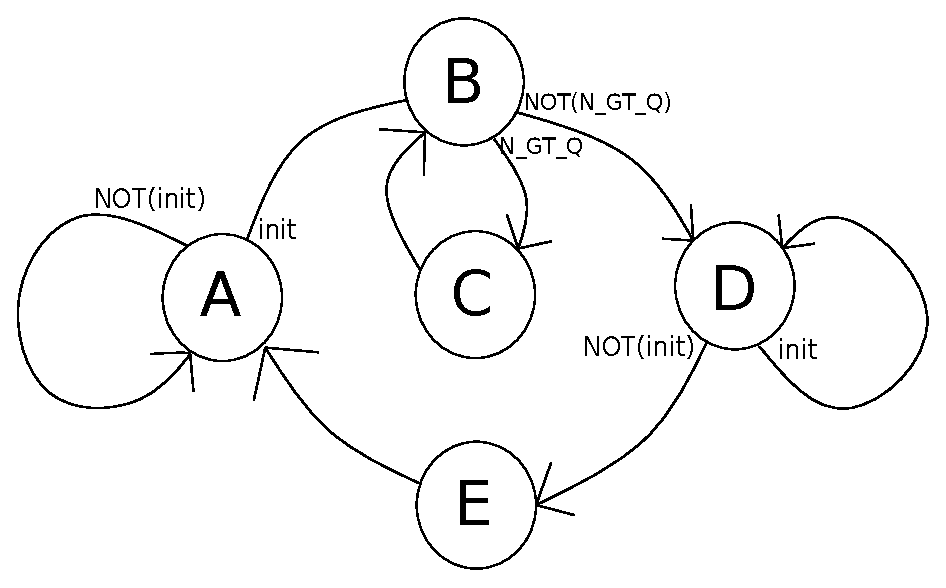
\includegraphics[scale=.6]{diag_5.eps}
	\caption{Machine state diagram}
	\label{fig:diag_state_5}
\end{figure}

\subsection{Question 3}

The basic principle behind a sequencer is that it is a chip that takes in a lot of conditions, all behind a multiplexer, and the sequence counter determines which one is selected to act either as a jumping trigger, or an increment trigger.

Two of these conditions have to be fixed at $1$ for ``unconditional load'' and $0$ for ``unconditional increase``.
Our conditions here are the triggers for our state changes, i.e. $\overline{init}$, $init$ and $\overline{N\_GT\_Q}$.

We obtain the following circuit in \autoref{fig:sequencer}.
\begin{figure}
	\centering
	\includegraphics[scale=.6]{machine_seq.png}
	\caption{Sequencing circuit}
	\label{fig:sequencer}
\end{figure}

The size of the jump code is determined by the selection width for the multiplexer, and the address is the consequence of choices made in the next question (because that address depends on how many codes total there are, and we need to code that to know it).

\subsection{Question 4}

Finally, let us create a microcode language for the control unit. Let us consider that we need at least $3$ bits in our messages for the next word selection, and $7$ bits for commands we send to the processing unit. If we consider that we have $5$ states to encode, with two loops, we get $5$ commands to encode in our ROM, and thus $3$ addressing bits necessary, so $7+3+3=13$ bits total.

Let's consider that the last three bits are the jump code for the sequencer to select the correct condition. Then the two bits before give a possible jump address in the ROM, and finally the first seven bits for all of our instructions.

And finally, we need to code.

In state $A$, is long as we detect $init$ (jump code $1$ on the sequencer), we jump to address $0$ (we stay in place), otherwise we will automatically jump to the next state we want with an increment. In this state, $RES0$ and $RESET$ are set to $1$, and the other controls to $0$. The first code is
\[
	\underbrace{001}_{\text{jump code}}\overbrace{000}^{\text{jump address}}\overbrace{0001001}_{\text{command codes}}
\]

In state $B$, if we detect that $\overline{N\_GT\_Q}$ (jump code $2$ on the sequencer), we jump to address $3$, otherwise we automatically jump to the next state we want with an increment (that'd mean we stay in the loop). In this state, nothing is turned on. The second code is
\[
	010~011~0000000
\]

In state $C$, we unconditionally jump back (jump code $7$ on the sequencer) to the address $1$, to evaluate the new condition. In this state, only $N1\_2\_N0$, $SUM\_N1$ and $INC\_Q$ are set to $1$.
\[
	111~001~1110000
\]

In state $D$, as long as we detect $init$ (jump code $1$ on the sequencer), we jump to address $3$ (we stay in place again), otherwise we will automatically jump to the next state we want with an increment. In this state, $RES1$ and $OUT_N0$ are set to $1$ while all of the other commands are set to $0$.
\[
	001~011~0000110
\]

In state $E$, we unconditionally jump to state $A$ (jump code 7 on the sequencer). In this state, $RES0$ is set to $1$ and everything else is set to $0$. The final sequence is
\[
	111~000~0001000
\]

And we get the microcode we want, assemble everything together, and we're good to go. See \autoref{fig:machine_cu} and \autoref{fig:machine_main} for the last pieces of assembly.

\begin{figure}
	\centering
	\includegraphics[scale=.5]{machine_cu.png}
	\caption{Command Unit for the machine}
	\label{fig:machine_cu}
\end{figure}

\begin{figure}
	\centering
	\includegraphics[scale=.5]{machine_main.png}
	\caption{Main circuit for the machine}
	\label{fig:machine_main}
\end{figure}


\end{document}
